\documentclass[11pt,a4paper]{article}

\usepackage[margin=1in]{geometry}
\usepackage{titlesec}
\usepackage{enumitem}
\usepackage{hyperref}
\usepackage{parskip}
\usepackage{graphicx}
\usepackage{float}
\usepackage{booktabs}
\usepackage{amsmath}

\hypersetup{colorlinks=true, linkcolor=blue, urlcolor=blue}

\titleformat{\section}{\large\bfseries}{\thesection}{0.5em}{}
\titleformat{\subsection}{\normalsize\bfseries}{\thesubsection}{0.5em}{}
\setlist{leftmargin=1.4em, topsep=2pt, itemsep=2pt}

\title{\vspace{-1.5cm}\textbf{PKCERT AI \& Software Development Internship \\ Task 10: Cross-Validation \& Hyperparameter Tuning}}
\author{Abdullah Amir}
\date{AI and Software Development \\ 15 July 2026}

\begin{document}

\maketitle
\vspace{-0.8cm}

This report covers the theory and the results. The full code, outputs and plots live
in the notebook \texttt{cv\_tuning.ipynb}. The dataset is \textbf{HTRU2}: 17,898
pulsar \emph{candidates} picked up by the High Time Resolution Universe radio survey.
Pulsars are a rare kind of rapidly rotating neutron star, and almost every detection a
radio telescope makes is actually interference or noise, so a human has to sift the
real ones out by hand. That is the job we are automating. Each candidate is described
by 8 continuous features and only \textbf{9.2 percent} of them are real pulsars. That
imbalance drives every decision in this report, including the one that matters most:
we tune on F1 rather than accuracy, because a model that labelled everything noise
would already score 91 percent accuracy without learning a thing.

% ----------------------------------------------------------------
\section*{Part A: Dataset Preparation}

\textbf{The features.} Each candidate signal is summarised twice over. The first four
features are the mean, standard deviation, excess kurtosis and skewness of the
\textbf{integrated pulse profile}, which is the signal averaged across many rotations.
The remaining four are the same four statistics taken from the \textbf{DM-SNR curve},
which describes how the signal strength varies with dispersion measure. The target
\texttt{Class} is 1 for a confirmed pulsar and 0 for noise, and every row has been
checked by a human annotator.

The data arrives genuinely clean: no missing values, no categorical columns to encode,
and a target that is already 0/1. So preparation comes down to two decisions.

\textbf{A stratified split.} We hold out 20 percent for testing and stratify on the
target, which leaves 14,318 candidates for training and 3,580 for testing, both
keeping the 9.2 percent pulsar rate. With a minority class this small, a careless
unstratified split could hand one side an unrepresentative slice and quietly poison
every number that follows.

\textbf{No scaling, on purpose.} This is the interesting one. In Task 09 scaling was
essential, because SVM and kNN both measure distances and a feature with a huge range
drowns out the rest. Here we use a Random Forest, and a tree splits on one feature at
a time by asking whether a value sits above some threshold. That question does not
care what units the feature is in, so tree ensembles are scale invariant and
standardising would change literally nothing. Skipping it is the correct call, not a
shortcut.

\begin{figure}[H]
    \centering
    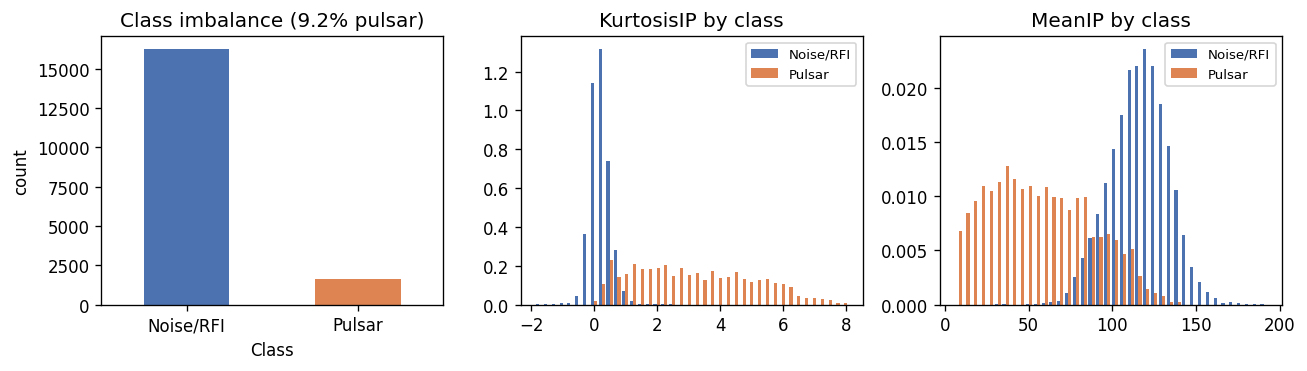
\includegraphics[width=0.95\textwidth]{figures/01_dataset_overview.png}
    \caption{Left: the 9.2 percent class imbalance that shapes the whole task. Middle
    and right: two features by class. The excess kurtosis of the integrated profile
    separates pulsars from noise almost cleanly on its own, which is why this problem
    is learnable at all.}
\end{figure}

% ----------------------------------------------------------------
\section*{Part B: Cross-Validation}

\textbf{The baseline.} We first train a Random Forest on stock scikit-learn defaults,
so that everything we do later has something honest to be measured against. A Random
Forest is a good fit here: it is an ensemble of decision trees, each grown on a
bootstrap sample of the rows and allowed to consider only a random subset of features
at each split, and averaging their votes cancels out most of the noise a single tree
would suffer from.

\textbf{Why cross-validate.} A single train/test split gives you exactly one number,
and that number depends on which rows happened to land in the test set.
\textbf{K-Fold cross-validation} fixes this by splitting the training data into K
parts, training on K-1 of them and validating on the one held back, then rotating so
every row gets validated exactly once. You end up with K scores instead of one, and
crucially you get their \emph{spread}, which tells you how much to trust any single
result. We use \textbf{StratifiedKFold} with K = 5, so each fold preserves the 9.2
percent pulsar rate. Plain KFold would be a real risk here: a fold could end up with
barely any pulsars, and its F1 would be noise.

\begin{table}[H]
\centering
\begin{tabular}{lrr}
\toprule
\textbf{Metric} & \textbf{Mean across 5 folds} & \textbf{Std} \\
\midrule
Accuracy & 0.9798 & 0.0026 \\
F1       & 0.8843 & 0.0162 \\
\bottomrule
\end{tabular}
\caption{5-fold cross-validation of the baseline Random Forest on the training set.}
\end{table}

\begin{figure}[H]
    \centering
    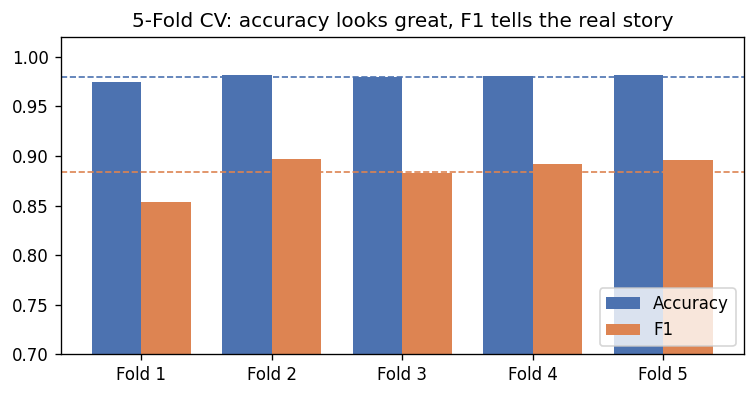
\includegraphics[width=0.62\textwidth]{figures/02_kfold_cv.png}
    \caption{Accuracy and F1 per fold. Accuracy is high and almost flat; F1 sits lower
    and visibly bounces around. The dashed lines are the means.}
\end{figure}

\textbf{Interpreting the results.} Two things jump out, and both matter for Part C.

First, \textbf{accuracy is flattering and close to useless here}. It averages 0.9798
with a tiny standard deviation of 0.0026, which looks like a triumph until you
remember that always guessing ``noise'' scores 0.908 for free. Accuracy is measuring
how well we handle the easy majority class, which is not the question anyone is
asking.

Second, \textbf{F1 is the honest number, and it is far wobblier}. It averages 0.8843
with a standard deviation of 0.0162, roughly six times accuracy's spread. That is
exactly what you would expect: each fold contains only about 260 pulsars, so a handful
of extra misses visibly moves the score. This spread is also the yardstick we carry
into the tuning stage. \emph{Any improvement smaller than about 0.016 is inside the
fold-to-fold noise and should not be believed.} That single observation turns out to
be the key to reading Part C correctly.

For those reasons we tune on \textbf{F1, not accuracy}. Optimising accuracy would
barely distinguish the candidates from one another.

% ----------------------------------------------------------------
\section*{Part C: Hyperparameter Tuning}

\textbf{GridSearchCV} tries every combination in a grid, exhaustively. Our grid varies
\texttt{n\_estimators} (100, 300), \texttt{max\_depth} (None, 10, 20),
\texttt{min\_samples\_leaf} (1, 2, 4), \texttt{max\_features} (sqrt, log2) and
\texttt{class\_weight} (None, balanced). That is $2\times3\times3\times2\times2 = 72$
combinations, each cross-validated over 5 folds, so \textbf{360 model fits}. It took
\textbf{456.5 seconds} and settled on \texttt{class\_weight='balanced'},
\texttt{max\_depth=None}, \texttt{max\_features='log2'}, \texttt{min\_samples\_leaf=2}
and \texttt{n\_estimators=300}, for a best cross-validated F1 of \textbf{0.8928}.

\textbf{RandomizedSearchCV} instead samples a fixed number of candidates from
\emph{distributions}. This lets us define a much wider space, with
\texttt{n\_estimators} drawn from anywhere in 50 to 400 rather than just two values,
plus extra options for \texttt{min\_samples\_split} and
\texttt{class\_weight='balanced\_subsample'}, while still capping the bill: we draw 30
candidates, so \textbf{150 fits}. It took \textbf{325.2 seconds} and chose
\texttt{class\_weight='balanced\_subsample'}, \texttt{max\_depth=None},
\texttt{max\_features='log2'}, \texttt{min\_samples\_leaf=1},
\texttt{min\_samples\_split=8} and \texttt{n\_estimators=111}, for a best
cross-validated F1 of \textbf{0.8899}.

\textbf{Comparing the optimal parameters.} The reassuring part is that both searches
landed in the \emph{same neighbourhood} despite exploring quite differently. Both
picked \texttt{max\_features='log2'}, both left the trees fully grown with
\texttt{max\_depth=None}, and, most tellingly, both chose a \emph{balanced} class
weight, which tells the forest to pay proportionally more attention to the rare
pulsars. Where they differ, 300 trees against 111, leaf size 2 against 1, the choices
are close to interchangeable in effect, which is itself a useful finding: this model
is not sensitive to those knobs on this data.

\begin{figure}[H]
    \centering
    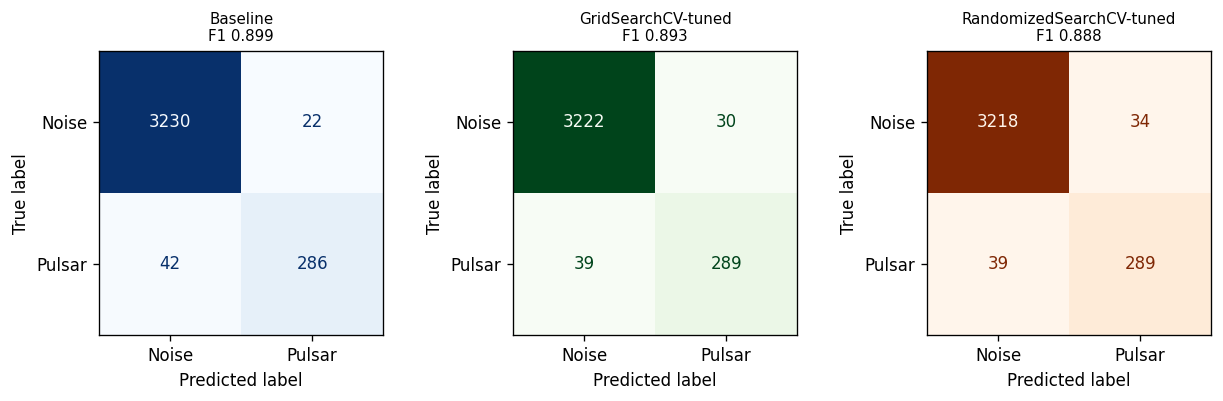
\includegraphics[width=0.95\textwidth]{figures/03_confusion_matrices.png}
    \caption{Confusion matrices for all three models. Rows are the true class, columns
    the prediction. Both tuned models catch 289 pulsars against the baseline's 286,
    and pay for it with a few more false alarms.}
\end{figure}

% ----------------------------------------------------------------
\section*{Part D: Comparative Analysis}

\begin{table}[H]
\centering
\begin{tabular}{lrrrrr}
\toprule
\textbf{Model} & \textbf{Accuracy} & \textbf{Precision} & \textbf{Recall} & \textbf{F1} & \textbf{ROC-AUC} \\
\midrule
Baseline (defaults)  & 0.9821 & 0.9286 & 0.8720 & 0.8994 & 0.9610 \\
GridSearchCV         & 0.9807 & 0.9060 & 0.8811 & 0.8934 & 0.9679 \\
RandomizedSearchCV   & 0.9796 & 0.8947 & 0.8811 & 0.8879 & 0.9690 \\
\bottomrule
\end{tabular}
\caption{Test-set metrics for the baseline and both tuned models.}
\end{table}

\begin{figure}[H]
    \centering
    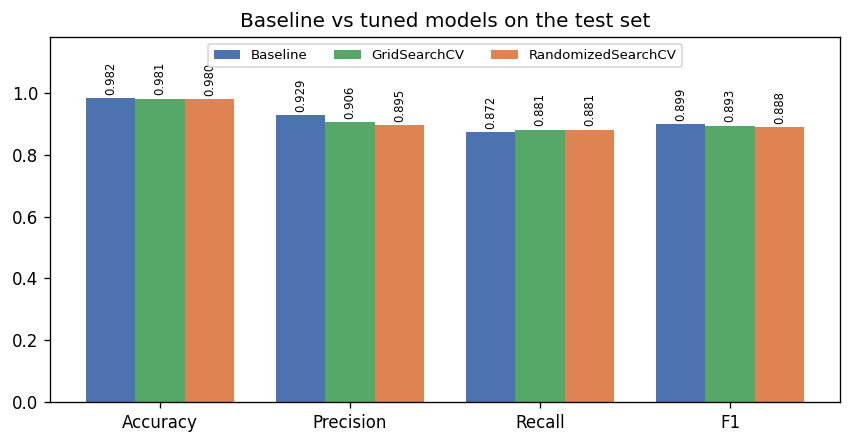
\includegraphics[width=0.66\textwidth]{figures/04_model_comparison.png}
    \caption{The four headline metrics side by side. The models are within a whisker
    of each other everywhere except recall, where both tuned models pull ahead.}
\end{figure}

\textbf{Baseline against optimized: an honest reading.} Tuning improved the score it
was actually optimising and slightly hurt the test score. Cross-validated F1 rose from
the baseline's 0.8843 to 0.8928 with grid search and 0.8899 with randomized search,
yet on the held-out test set the \emph{baseline} posts the best F1 at 0.8994, against
0.8934 and 0.8879. That looks like a contradiction and it is not. It is simply what
tuning looks like when the defaults are already good, and there are three things going
on underneath.

\begin{itemize}
    \item \textbf{Every gap is inside the noise.} Part B measured the fold-to-fold
    standard deviation of F1 at 0.0162. All of these differences are around 0.006 to
    0.01, comfortably smaller. Statistically we cannot separate these three models,
    and pretending otherwise would be reading tea leaves.
    \item \textbf{The searches traded precision for recall, deliberately.} Both picked
    a balanced class weight, which pushes the forest to work harder on the rare class.
    It did exactly that: recall climbed from 0.8720 to 0.8811, catching 3 more real
    pulsars (286 up to 289), at a cost in precision from 0.9286 to 0.9060, meaning 8
    more false alarms. F1 weighs those two equally, so it came out marginally down.
    \item \textbf{Ranking quality genuinely improved.} ROC-AUC rose from 0.9610 to
    0.9679 and 0.9690. Unlike F1 it does not depend on where you put the 0.5
    threshold, so it says the tuned models really do order candidates better, which is
    a real gain the F1 column hides.
\end{itemize}

\textbf{Which model would I actually ship?} The tuned one, in spite of the lower F1.
In pulsar astronomy a missed pulsar is a lost discovery, while a false alarm costs an
astronomer a couple of minutes of eyeballing. Recall and ranking quality matter more
here than F1's symmetric view of the two errors, and the tuned models win on both.

\textbf{Advantages and limitations of the two searches.}

\begin{itemize}
    \item \textbf{GridSearchCV.} Exhaustive, fully reproducible, and guaranteed to
    find the best point \emph{in the grid you wrote}. That guarantee is worth less
    than it first sounds, because you only ever find what you thought to list. Its
    real problem is combinatorial: adding one parameter with three values triples the
    cost, and it keeps spending fits on parameters that turn out not to matter. It
    also cannot search a continuous range at all.
    \item \textbf{RandomizedSearchCV.} Its cost is set by \texttt{n\_iter}, not by the
    size of the space, so you decide the budget up front. It samples continuous
    distributions and copes with many parameters at once, which is why it scales where
    grid search does not. The trade is that it offers no guarantee of hitting the
    optimum, its result shifts with the random seed, and \texttt{n\_iter} is one more
    thing you have to choose.
\end{itemize}

\begin{figure}[H]
    \centering
    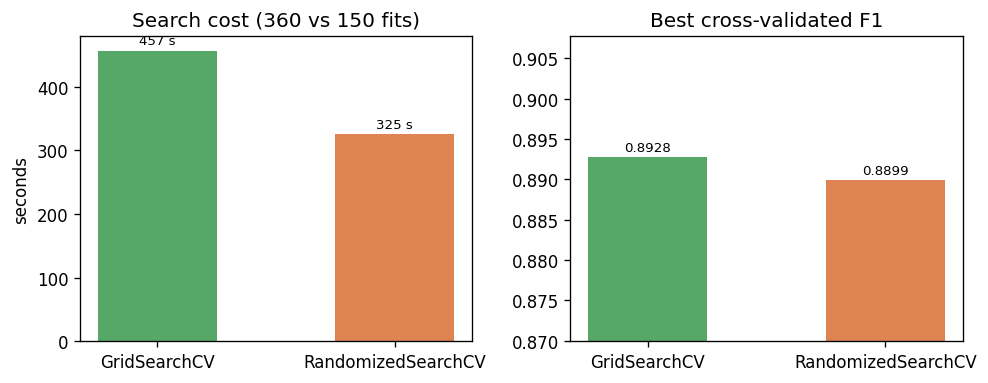
\includegraphics[width=0.78\textwidth]{figures/05_search_comparison.png}
    \caption{Cost against payoff. Randomized search reached a statistically
    indistinguishable F1 for well under half the fits.}
\end{figure}

Concretely: grid ran 360 fits in 456.5 seconds for a CV F1 of 0.8928, randomized ran
150 fits in 325.2 seconds for 0.8899. Randomized search got within \textbf{0.3
percent} of grid's score using \textbf{42 percent} of the fits. One honest caveat
worth flagging: the time saving (1.4 times) is smaller than the fit saving (2.4
times), because the wider space let randomized search sample genuinely expensive
configurations that grid never tried, such as \texttt{max\_features=None} and forests
of up to 400 trees. Fewer fits does not automatically mean proportionally less time.

A note on those timings. The seconds quoted here and plotted above come from the run
of \texttt{cv\_tuning.py} that also produced the figures. Wall clock timings depend on
the machine and on whatever else it is doing at the time, so they are not exactly
reproducible: the notebook run of the same code, executed while the laptop was busy
compiling this report, took 852 and 417 seconds for the same two searches. The
\emph{fit counts} (360 against 150) and every metric are fixed by the code and the
random seeds, so those are the numbers to judge the two searches on. Reassuringly, the
conclusion does not move either way, randomized search came out roughly 1.4 to 2 times
quicker in both runs.

\textbf{Recommendation.} \emph{RandomizedSearchCV is the more suitable approach for
this dataset}, and it is the better default in general. It matched grid search to
within noise for well under half the compute, and explored a wider space while doing
it. The practical recipe this points to is a two-stage one: start with
RandomizedSearchCV over a deliberately wide space to find the promising region
cheaply, then, only if the payoff justifies the time, run a small GridSearchCV around
the winner to polish. Pure grid search earns its keep only when the space is small and
discrete enough that the whole thing is genuinely affordable.

And the headline finding, stated plainly: \emph{on this dataset, tuning was not worth
much}. The Random Forest defaults were already close to optimal, and a quarter of an
hour of searching bought slightly better recall and ranking rather than any real jump
in performance. That is a perfectly normal outcome and a useful one to be able to
recognise. Knowing when tuning has nothing left to give is as valuable a skill as the
tuning itself, and it is a good deal more honest than presenting a 0.006 wobble as an
improvement.

\vspace{0.4cm}
The notebook and README are on GitHub:
\url{https://github.com/AbdullahAmir06/ai-internship-abdullahamir}.

\end{document}